\section{Diodo 1N4007: caratteristica volt-amperometrica}

\begin{wrapfigure}[25]{r}[0pt]{130mm}
	\label{fig:diodo}
	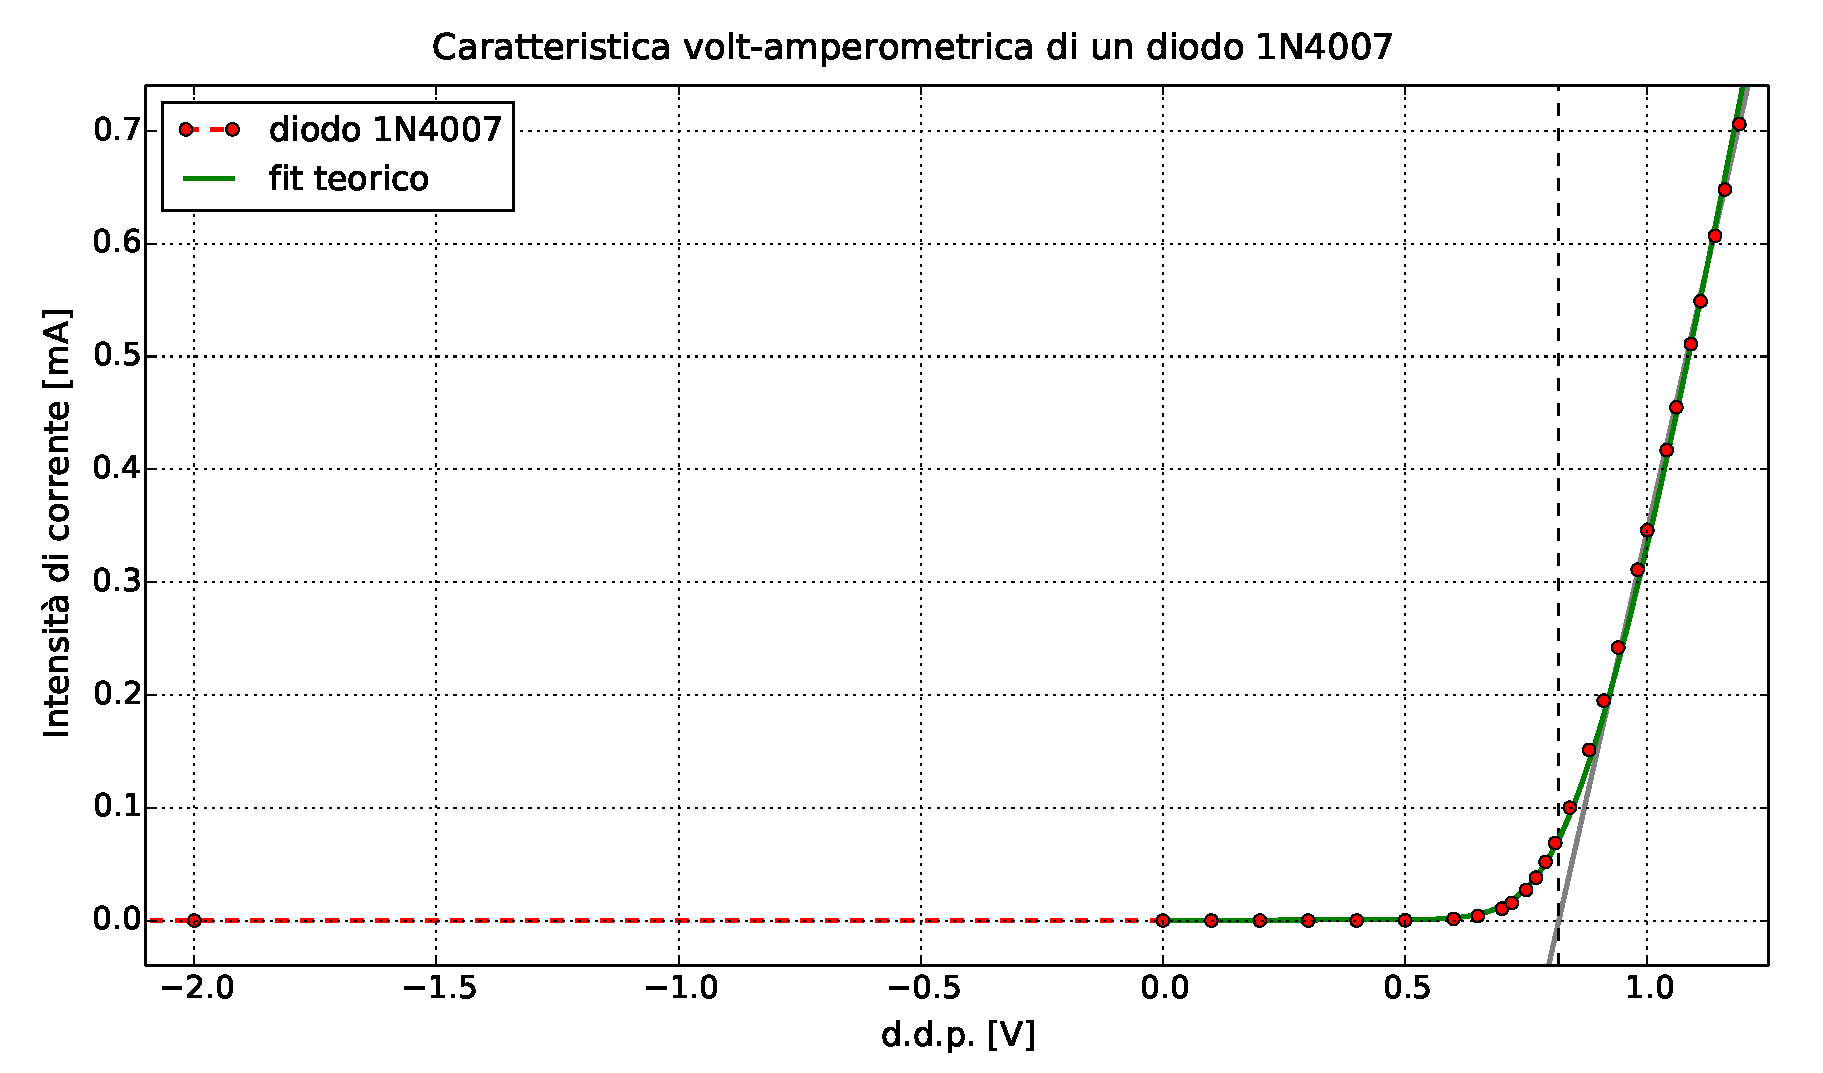
\includegraphics[width=0.75\textwidth]{diodo.pdf}
	\caption{I dati rappresentati non sono il set intero, che arriva fino a $\SI{-50}{\volt}$, bensì solo i più significativi. Questa scelta è stata effettuata sia per necessità di spazio che per, soprattutto, leggibilità del grafico. Per completezza $I(\SI{-50.06}{\volt}) = \SI{-12}{\nano\ampere}$. Inoltre, $V_d = (0.82 \pm 0.02)\,\si{\volt}$.}
	\label{fig:diodo}
\end{wrapfigure}

Per studiare la caratteristica volt-amperometrica del diodo abbiamo dovuto separare l'analisi in due fasi distinte: una prima fase in cui abbiamo analizzato il comportamento del diodo polarizzato in diretta e una seconda fase in cui ne abbiamo analizzato il comportamento in inversa.
Utilizzando la breadboard come supporto, abbiamo creato un circuito composto dal genertore di tensione continua (max $\pm \SI{25}{\volt}$), il diodo e il multimetro digitale in modalità amperometro. Aumentando progressivamente la tensione, abbiamo letto sull'amperometro i valori della corrente che attraversava il circuito.
Facendo attenzione che la corrente non superasse il valore di \SI{700}{\milli\ampere}\footnote{Abbiamo impostato il fondo scala dell'amperometro ad 1 ampere. Sulle specifiche dello strumento risulta che la resistenza interna dello strumento è pari a $R=0.1 \Omega$} abbiamo quindi popolato l'asse positivo del grafico. In seguito abbiamo girato il diodo in modo che fosse alimentato in inversa e abbiamo popolato anche l'asse negativo del grafico, ottenendo la caratteristica volt-amperometrica completa del diodo. Il risultato è esposto in Fig. \ref{fig:diodo}. 

\phantom{x}

Osserviamo innanzitutto che il valore di caduta di tensione diretta da noi ricavato è di $(0.82 \pm 0.02)\,\si{\volt}$.\\
Riportiamo ora la legge teorica della caratteristica V-I di un diodo al silicio:
\begin{equation}
I_{D} \, = \, I_{S} \left( e^{\frac{q V_d}{nKT}} -1 \right)
\label{eq:diode}
\end{equation}
Dove $I_S$ è la corrente di saturazione, $q$ la carica dell'elettrone, $K$ la costante di Boltzmann, $T$ la temperatura assoluta e $n$ il fattore di idealità. 
Notiamo come il diodo, per una tensione superiore a quella di soglia, si comporti quasi come un conduttore ideale, ovvero faccia scorrere grandi correnti per piccole variazioni di tensione. 

Abbiamo tentato un fit con una legge del tipo : 

\begin{equation}
I_{D} \, = \, \alpha \left( e^{\frac{V_{D}}{B}} -1 \right)
\label{eq:diodefit}
\end{equation}

Nonostante i nostri tentativi, non siamo riusciti a trovare dei valori per i parametri $\alpha$ e $B$ tali per cui la legge fittasse correttamente i dati. Abbiamo dunque pensato che ciò fosse causato dalla resistenza interna dell'amperometro. Abbiamo dunque impostato la seguente equazione:

$$V=I_D \cdot R + V_D$$

Con $V$ la tensione fornita dal generatore e $R$ la resistenza delle componenti circuitali escluso il diodo. Da Eq.(\ref{eq:diodefit}) troviamo immediatamente la seguente equazione:

\begin{equation}
V=I_D \cdot R + B \cdot ln (\frac{I_D+\alpha}{\alpha})
\label{eq:diodefit2}
\end{equation}

Come vediamo, per poter fittare i nostri dati dobbiamo o invertire la caratteristica V-I o la funzione appena trovata. Poichè è complicato operare quest'ultima possibilità, abbiamo deciso di eseguire un fit tenendo la funzione implicita appena trovata. I valori dei parametri stimati sono $\alpha=(4\pm 5)\times 10^{-8} \,\si{\ampere}$, $B=(0.055\pm 0.005)\,V $ e $R=(0.37\pm 0.05)\,\si{\ohm}$.

Come vediamo dal grafico sopra riportato, i dati sembrano fittare la legge implicita ipotizzata. Notiamo anche che sul valore $\alpha$ abbiamo una grande incertezza percentuale (oltre il 100\%). Non è quindi preciso calcolare la corrente di saturazione $I_S$ eseguendo una procedura come quella da noi effettuata. Notiamo anche che il valore di $R$ calcolato risulta diverso dalla resistenza interna dell'amperometro riportata dal costruttore. Ciò probabilmente è dovuto al fatto che ci sono delle altre resistenze parassite di cui non si è tenuto conto. 
 
\section{Cella solare: caratteristica volt-amperometrica}

Abbiamo studiato la caratteristica volt-amperomentrica di una cella solare lavorando allo stesso modo di come abbiamo fatto per il diodo.
La prima analisi sul comportamento della cella è stata svolta tenendo la cella solare al buio nella sua scatola, mentre una seconda analisi è stata completata con la cella solare sottoposta alla radiazione di una lampada da tavolo, facendo attenzione che quest'ultima non variasse di intensità.
Dall'analisi dati abbiamo notato che la cella solare si comporta sostanzialmente come un diodo, eccetto nella polarizzazione in inversa, dove per tensioni di $-50V$ si hanno valori di corrente significativamente maggiori rispetto a quelli misurati nel caso del diodo semplice. 

Nella parte di analisi operata sotto la luce abbiamo notato che la cella fotovoltaica non cambia la forma della sua caratteristica V-I, ma vi è solo una traslazione: 

$$f'(V)=f(V)-25.5 \, [mA]$$ %controllare forse
 
%Durante questa parte dell'esperienza abbiamo avuto cura che la corrente massima da cui era attraversata la cella non superasse i \SI{100}{\milli\ampere}. 
I dati ottenuti sono graficati in Fig. \ref{fig:cella}.

\begin{figure}[h]
\center
	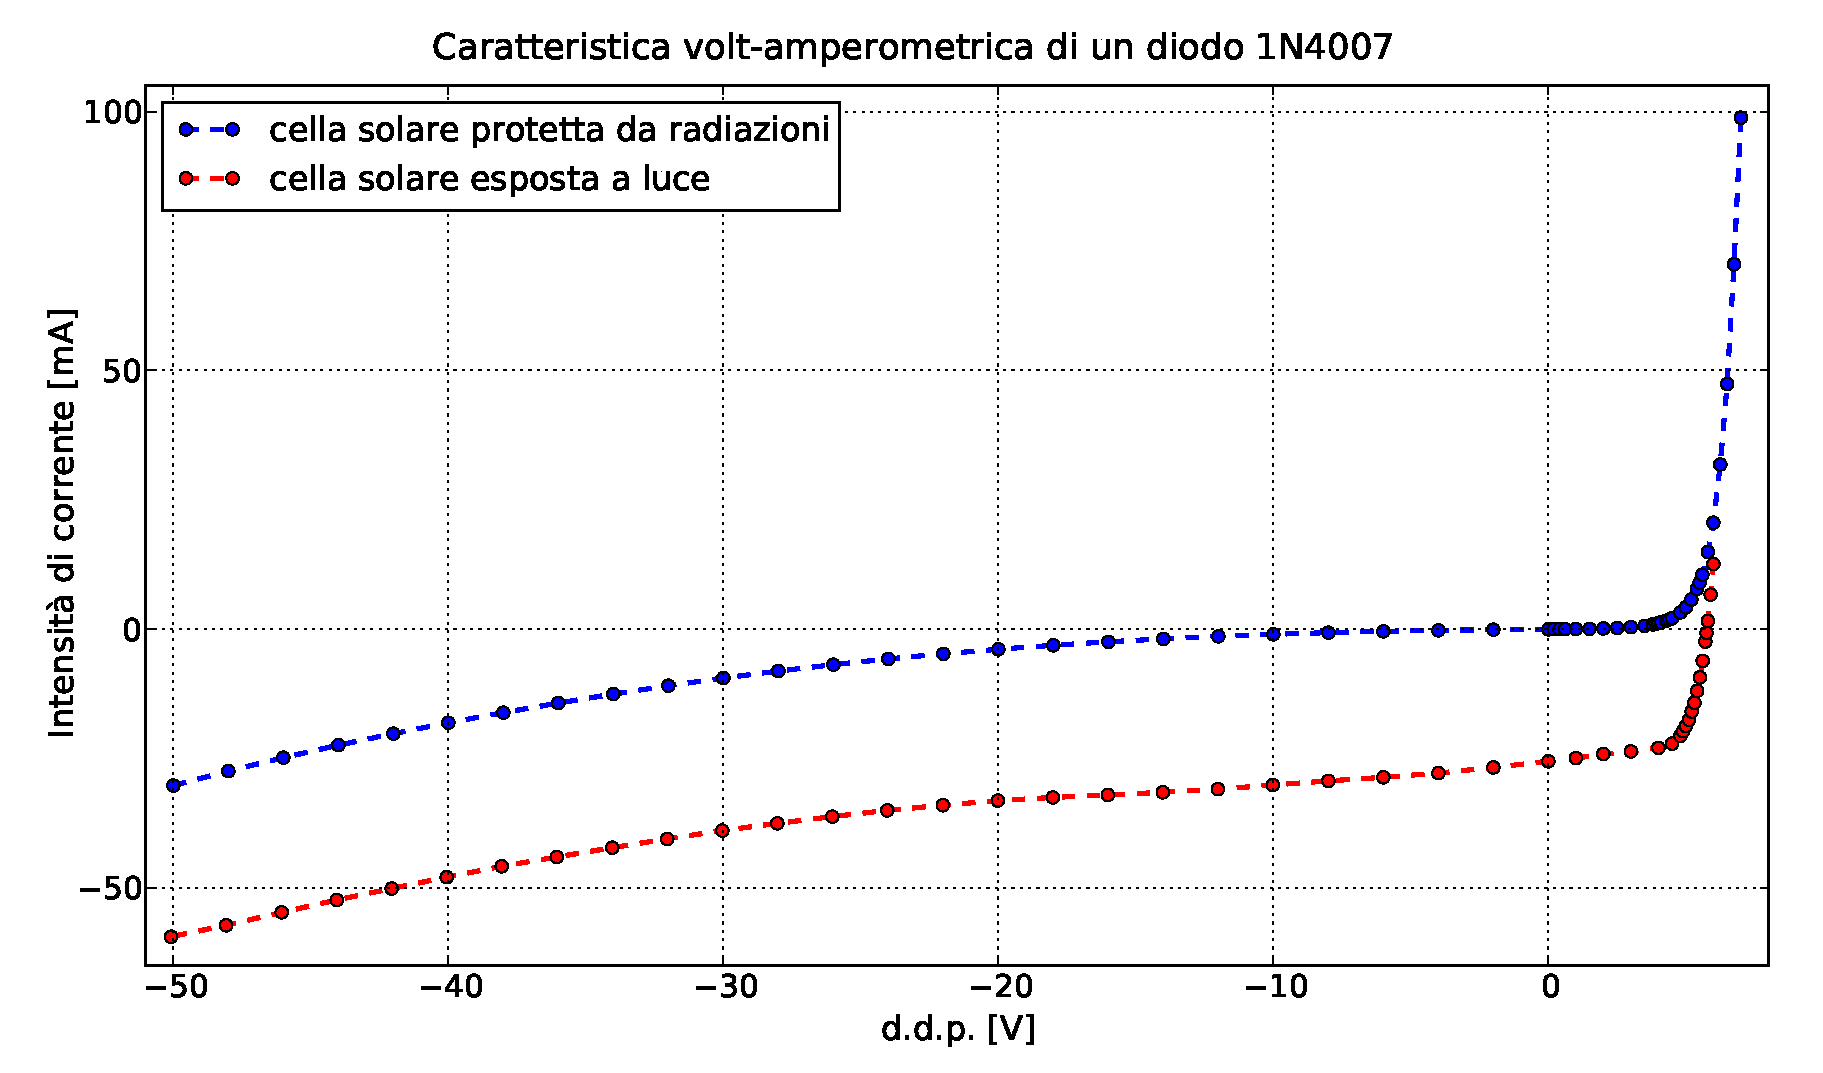
\includegraphics[width=0.75\textwidth]{cella.pdf}
	\caption{Caratteristica volt-amperometrica della cella solare al buio (punti blu) e alla luce (punti rossi). Sono evidenziati i valori di corrente e tensione definiti a potenza massima ($I_{@P_{max}}$ e $V_{@P_{max}}$), il valore di tensione a corrente nulla ($V_{oc}$) e il valore di corrente per tensione nulla ($I_{sc}$)}
	\label{fig:cella}
\end{figure}

Un'altra caratteristica della cella solare è il \emph{Fill Factor}. Questo è un parametro fondamentale nella valutazione delle prestazioni delle celle solari. Esso è definito come il rapporto tra l'effettiva potenza massima ottenibile e il prodotto della tensione a circuito aperto e la corrente di corto circuito.

\begin{equation}
FF \, = \, \frac{I_{@P_{max}} \,\, V_{@P_{max}}}{I_{sc} \,\, V_{oc}}
\label{eq:FF}
\end{equation}

Le celle con un alto Fill Factor hanno una bassa resistenza equivalente in serie e una elevata resistenza equivalente in parallelo, quindi più è elevato il Fill Factor meno corrente prodotta dalla cella viene dissipata in perdite interne.

Nel nostro caso il Fill Factor è risultato essere:

$$FF \,=\, 0.67 \pm 0.05$$
\section{Ponte di Graetz}

\begin{wrapfigure}[11]{r}[0pt]{65mm}
	\caption{Schema del ponte di Graetz da noi utilizzato. I quattro diodi sono uguali.}
	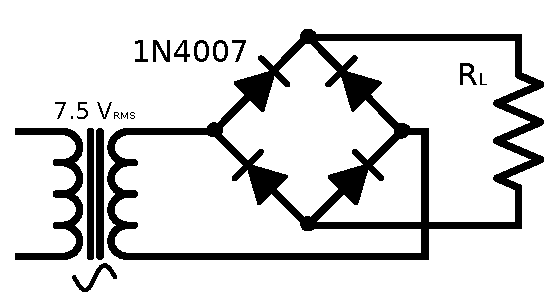
\includegraphics[width=0.35\textwidth]{schema_graetz.pdf}
	\label{fig:graetz}
\end{wrapfigure}

Un ponte costituito da diodi può essere utilizzato come elemento raddrizzatore di un segnale. Riportiamo in Fig. \ref{fig:graetz} lo schema del ponte di Graetz da noi utilizzato. Tale ponte permette di raddrizzare un segnale in entrata, ovvero di trasformarlo in un segnale non negativo e quindi fare in modo che un'uscita del ponte sia sempre positiva e l'altra negativa. Poichè i diodi hanno una caduta di tensione diretta, o tensione di soglia, il segnale raddrizzato non potrà superare in tensione massima la tensione del segnale in entrata. Infatti vi sarà sempre una certa differenza di potenziale tra il segnale in \emph{input} e il segnale raddrizzato a causa della caduta di tensione propria dei diodi tranne quando la tensione i entrata sarà inferiore al valore di soglia. In tale caso il segnale raddrizzato avrà tensione nulla.

Poichè l'oscilloscopio è collegato a massa, non è possibile visualizzare a schermo contemporaneamente sia segnale in input che segnale in uscita dal ponte. Si è dunque utilizzata la funzione integrata all'oscilloscopio $Permanenza$ che fa rimanere sullo schermo l'ombra dei segnali visualizzati. \`E stato così possibile osservare sull'oscilloscopio entrambi i segnali. Ricordiamo che la resistenza da noi utilizzata come carico aveva un valore di $R_L=9998 \pm 1$.

Nel seguente grafico sono riportati i segnali da noi visualizzati.

\begin{figure}[h]
\center
	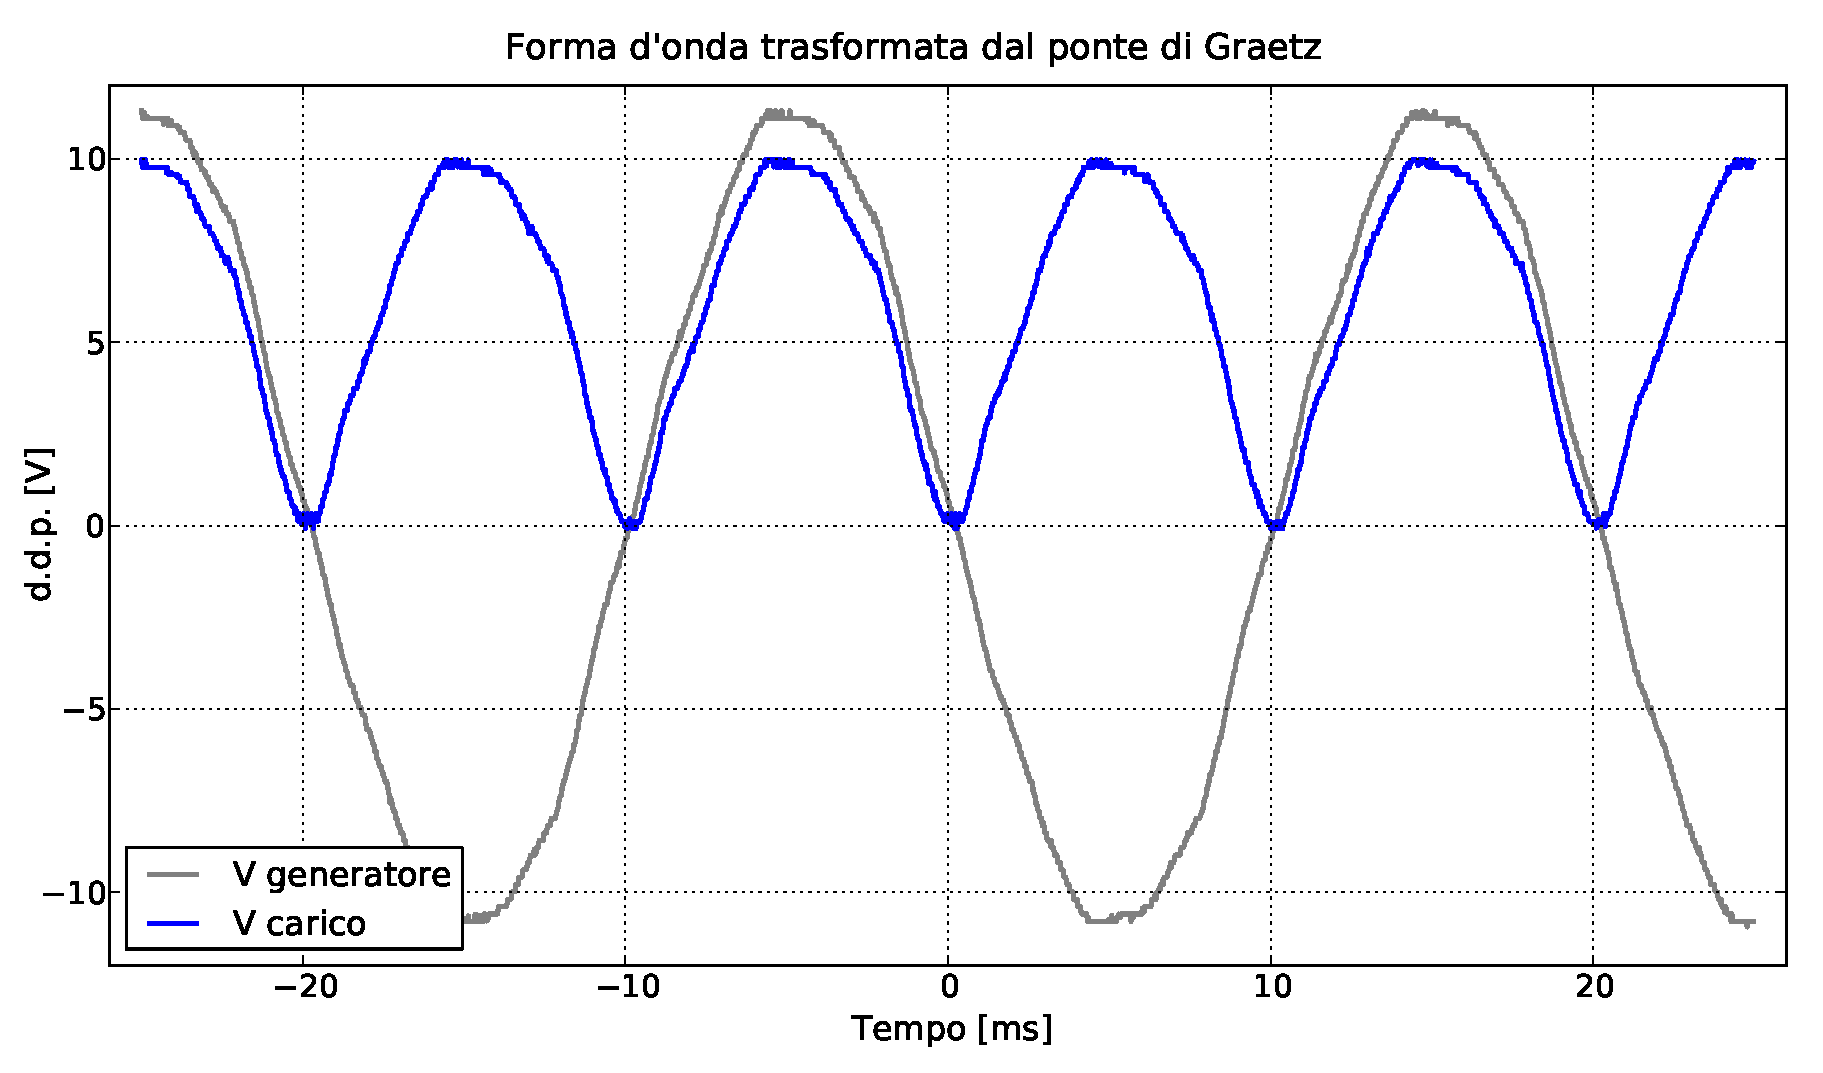
\includegraphics[width=0.75\textwidth]{graetz.pdf}
	\caption{In grigio è stato graficato il segnale in entrata al circuito, mentre il blu quello ai capi del carico. Come si può vedere il segnale in uscita dal ponte di Graetz è sempre positivo, ma l'ampiezza è ridotta a causa della caduta di tensione determinata dai diodi.}
	\label{fig:graetz}
\end{figure}

\begin{wrapfigure}[11]{r}[0pt]{65mm}
	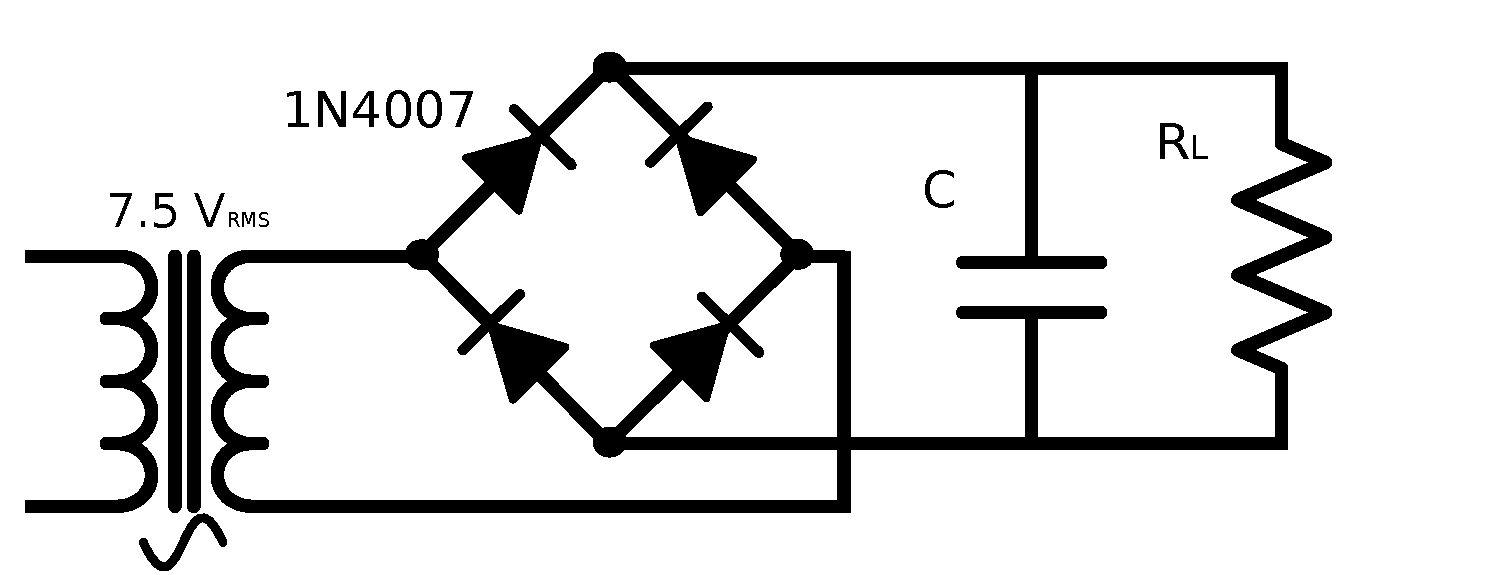
\includegraphics[width=0.4\textwidth]{schema_ripple.pdf}
	\caption{Schema del ponte di Graetz con condensatore, per stabilizzare il segnale in output. Ancora una volta i quattro diodi sono uguali.}
	\label{fig:schema_ripple}
\end{wrapfigure}

Avendo utilizzato un segnale sinusoidale in input vediamo che per valori di $V \approx 0$ i diodi non sono in conduzione e dunque la d.d.p in output risulta nulla. \`E importante osservare come la frequenza del segnale in uscita sia raddoppiata. Infatti per ogni periodo della funzione sinusoidale fornita dal generatore abbiamo due periodi della funzione in uscita.

\phantom{x}

Una volta ottenuto il segnale raddrizzato, l'interesse si sposta sul modo di ottenere un segnale di tensione DC il più costante possibile. Per fare ciò abbiamo utilizzato un condensatore messo in parallelo al carico in uscita dal ponte di diodi, come riportato dallo schema in Fig. \ref{fig:schema_ripple}.

La capacità gioca un ruolo fondamentale in quanto, caricandosi e scaricandosi, manda in interdizione i diodi del ponte, causando una stabilizzazione del segnale su un valore medio che dipende dalla capacità stessa. Per valori di capacità $C\neq 0$ il valore medio di tensione in uscita dal ponte si sposta su valori più alti man mano che anche il valore di $C$ aumenta.
%Inoltre, la forma d'onda in uscita risulta tanto più simile ad una scarica/carica di un condensatore quanto più alto è il valore di capacità. SIAMO SICURI?
Il segnale che si vede a schermo, riportato in Fig. \ref{fig:ripple}, risulta dunque simile alla sovrapposizione di un segnale oscillante ad uno continuo. Tale fenomeno viene comunemente chiamato $Ripple$.

Si definisce il fattore di ripple come: $r_f= \frac{V_{AC}}{V_{DC}}$, dove $V_{AC}$ è la differenza picco-picco del segnale mentre $V_{DC}$ la sua media. Per calcolare $V_{DC}$ abbiamo utilizzato la funzione integrata dell'oscilloscopio che esegue una media integrale. Riportiamo in tabella i dati da noi ottenuti:

%\begin{SCtable}[20][h]
\begin{table}[H]
\center
\caption{Dati da noi registrati con relativi errori.}
{\renewcommand{\arraystretch}{1.6}%
\begin{tabular}{c|c|c|c|c}
Capacità [$\si{\nano\farad}$] & Frequenza [$\si{\hertz}$] & $V_{AC}$ ripple [$\si{\volt}$] & $V_{DC}$ [$\si{\volt}$] & $r_f$ \\      \hline
$401 \pm 2$ &$100.1 \pm 0.1 $& $6.93 \pm 0.01$ & $6.87 \pm 0.01$ & $1.01 \pm 0.02$\\
$799 \pm 5$ &$100.2 \pm 0.1$& $5.28 \pm 0.01$ & $7.57 \pm 0.01$ & $0.70 \pm 0.02$\\
$1196 \pm 5$ &$100.1 \pm 0.1$& $4.42 \pm 0.01$ & $8.06 \pm 0.01$ & $0.55 \pm 0.02$\\
$4959 \pm 3$ &$100.3 \pm 0.1$& $1.45 \pm 0.01$ & $9.25 \pm 0.01$& $0.16 \pm 0.02$\\
\end{tabular}}
\end{table}
%\end{SCtable}

Come ci aspettavamo, aumentando la capacità aumenta anche il valore $V_{DC}$. Inoltre vi è anche un sensibile smorzamento delle fluttuazioni del segnale attorno a tale valor medio. Per ottenere una tensione continua stabile è dunque preferibile utilizzare una capacità più grande possibile, così da minimizzare in fattore $r_f$.

Riportiamo infine un grafico dei segnali a schermo ottenuti per la capacità $C=\SI{1196}{\nano\farad}$. Come si può vedere, la forma d'onda in uscita non è più simile al valore assoluto del segnale in ingresso ma ad una serie di scariche/cariche di un condensatore.

\begin{figure}[h]
\center
	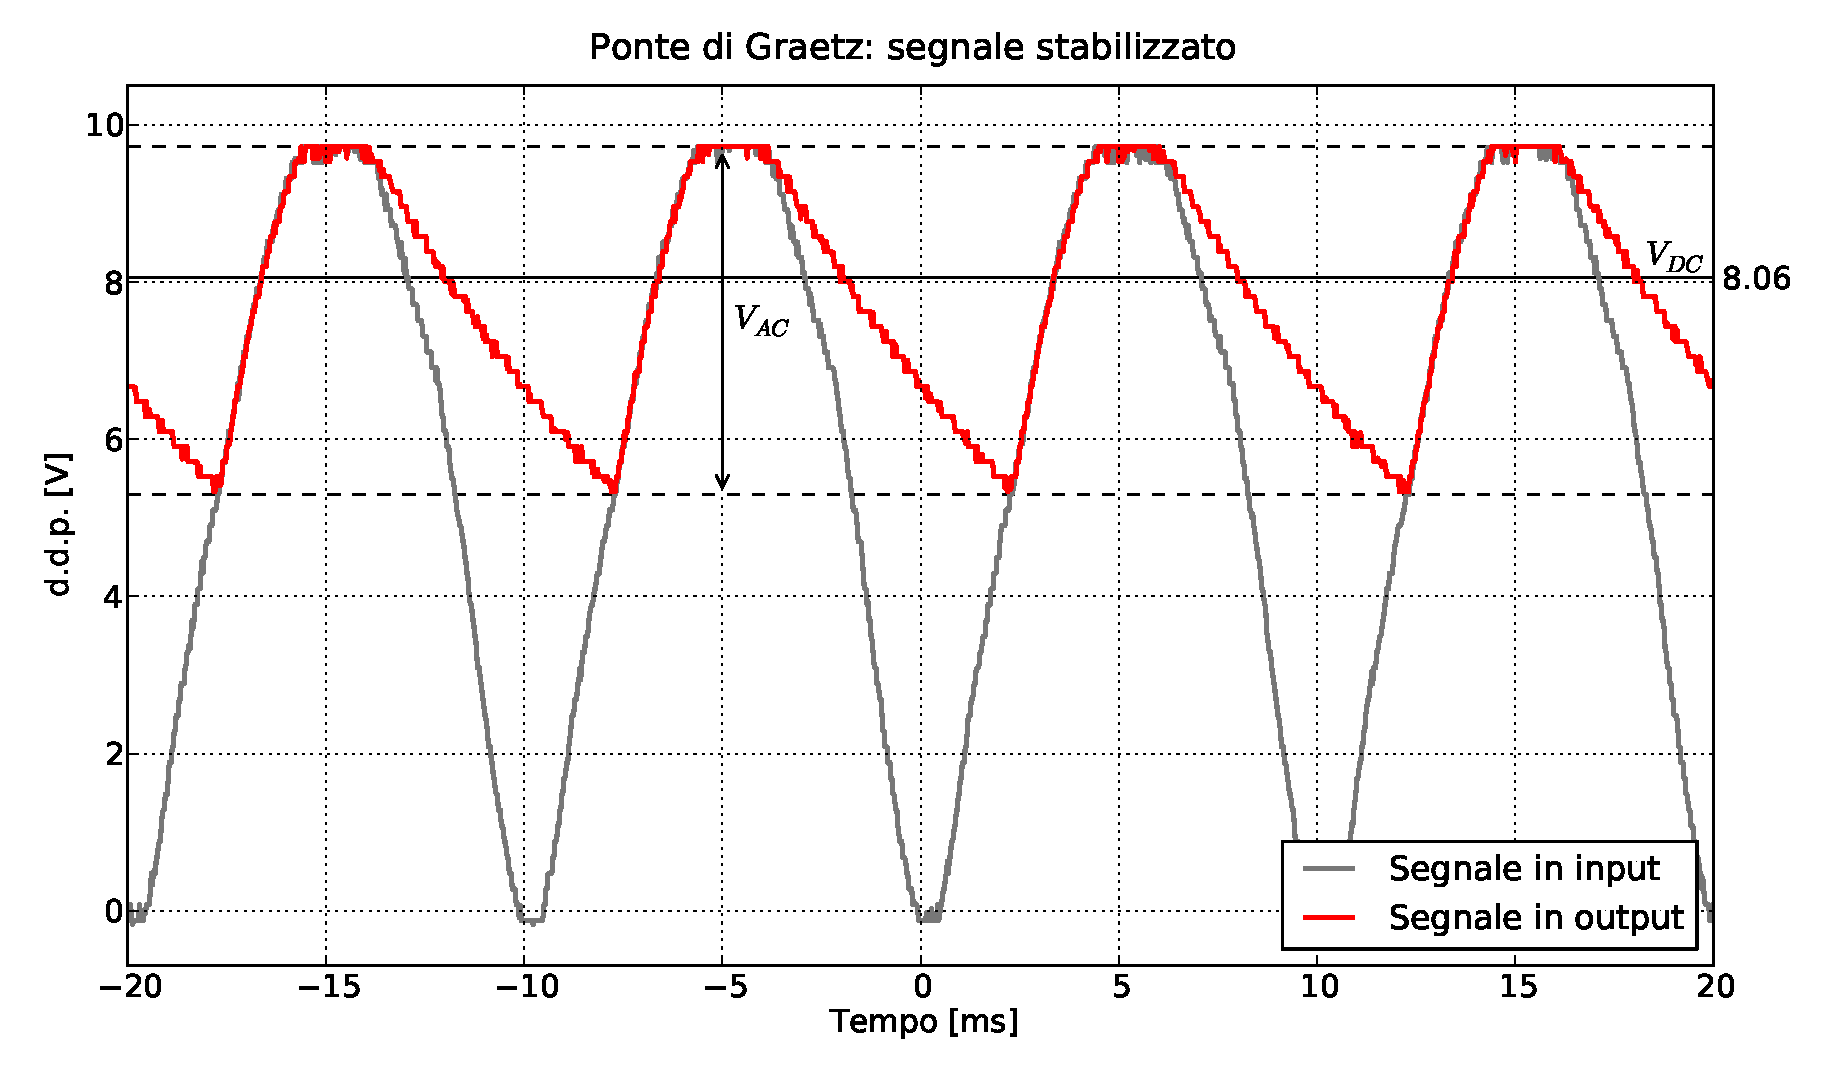
\includegraphics[width=0.75\textwidth]{ripple.pdf}
	\caption{In grigio possiamo apprezzare il segnale in ingresso al circuito, in verde in segnale in uscita dal ponte di Graetz senza il condensatore mentre in rosso vediamo quello ai capi del carico quando si aggiunge il condensatore.}
	\label{fig:ripple}
\end{figure}